\documentclass[journal,12pt,twocolumn]{IEEEtran}
%
\usepackage{setspace}
\usepackage{multicol}
\usepackage{gensymb}
\usepackage{enumerate}
\usepackage{xcolor}
\usepackage{caption}
%\usepackage{subcaption}
%\doublespacing
\singlespacing
%\usepackage{epstopdf}
%\usepackage{graphicx}
%\usepackage{amssymb}
%\usepackage{relsize}
\usepackage[cmex10]{amsmath}
\usepackage{mathtools}
%\usepackage{amsthm}
%\interdisplaylinepenalty=2500
%\savesymbol{iint}
%\usepackage{txfonts}
%\restoresymbol{TXF}{iint}
%\usepackage{wasysym}
\usepackage{amsthm}
\usepackage{mathrsfs}
\usepackage{txfonts}
\usepackage{stfloats}
\usepackage{cite}
\usepackage{cases}
\usepackage{subfig}
%\usepackage{xtab}
\usepackage{longtable}
\usepackage{multirow}
%\usepackage{algorithm}
%\usepackage{algpseudocode}
%\usepackage{enumitem}
\usepackage{mathtools}
\usepackage{iithtlc}
%\usepackage[framemethod=tikz]{mdframed}
\usepackage{listings}
\usepackage{amsmath}
\usepackage{polynomial}
\usepackage{url}
\def\UrlBreaks{\do\/\do-}
%\usepackage{stmaryrd}


%\usepackage{wasysym}
%\newcounter{MYtempeqncnt}
\DeclareMathOperator*{\Res}{Res}
%\renewcommand{\baselinestretch}{2}
\renewcommand\thesection{\arabic{section}}
\renewcommand\thesubsection{\thesection.\arabic{subsection}}
\renewcommand\thesubsubsection{\thesubsection.\arabic{subsubsection}}

\renewcommand\thesectiondis{\arabic{section}}
\renewcommand\thesubsectiondis{\thesectiondis.\arabic{subsection}}
\renewcommand\thesubsubsectiondis{\thesubsectiondis.\arabic{subsubsection}}

% correct bad hyphenation here
\hyphenation{op-tical net-works semi-conduc-tor}

\lstset{
language=Python,
frame=single, 
breaklines=true
}

%\lstset{
	%%basicstyle=\small\ttfamily\bfseries,
	%%numberstyle=\small\ttfamily,
	%language=python,
	%backgroundcolor=\color{white},
	%%frame=single,
	%%keywordstyle=\bfseries,
	%%breaklines=true,
	%%showstringspaces=false,
	%%xleftmargin=-10mm,
	%%aboveskip=-1mm,
	%%belowskip=0mm
%}

%\surroundwithmdframed[width=\columnwidth]{lstlisting}


\begin{document}
%

\theoremstyle{definition}
\newtheorem{theorem}{Theorem}[section]
%\newtheorem{problem}{Problem}[section]
\newtheorem{problem}{Problem}
\newtheorem{proposition}{Proposition}
%\newtheorem{proposition}{Proposition}[section]
\newtheorem{lemma}{Lemma}[section]
\newtheorem{corollary}[theorem]{Corollary}
\newtheorem{example}{Example}[section]
%\newtheorem{definition}{Definition}[section]
\newtheorem{definition}{Definition}
%\newtheorem{definition}{Definition}
%\newtheorem{algorithm}{Algorithm}[section]
%\newtheorem{cor}{Corollary}
\newcommand{\BEQA}{\begin{eqnarray}}
\newcommand{\EEQA}{\end{eqnarray}}
\newcommand{\define}{\stackrel{\triangle}{=}}

\bibliographystyle{IEEEtran}
%\bibliographystyle{ieeetr}

\providecommand{\nCr}[2]{\,^{#1}C_{#2}} % nCr
\providecommand{\nPr}[2]{\,^{#1}P_{#2}} % nPr
\providecommand{\mbf}{\mathbf}
\providecommand{\pr}[1]{\ensuremath{\Pr\left(#1\right)}}
\providecommand{\qfunc}[1]{\ensuremath{Q\left(#1\right)}}
\providecommand{\sbrak}[1]{\ensuremath{{}\left[#1\right]}}
\providecommand{\lsbrak}[1]{\ensuremath{{}\left[#1\right.}}
\providecommand{\rsbrak}[1]{\ensuremath{{}\left.#1\right]}}
\providecommand{\brak}[1]{\ensuremath{\left(#1\right)}}
\providecommand{\lbrak}[1]{\ensuremath{\left(#1\right.}}
\providecommand{\rbrak}[1]{\ensuremath{\left.#1\right)}}
\providecommand{\cbrak}[1]{\ensuremath{\left\{#1\right\}}}
\providecommand{\lcbrak}[1]{\ensuremath{\left\{#1\right.}}
\providecommand{\rcbrak}[1]{\ensuremath{\left.#1\right\}}}
\theoremstyle{remark}
\newtheorem{rem}{Remark}
\newcommand{\sgn}{\mathop{\mathrm{sgn}}}
\providecommand{\abs}[1]{\left\vert#1\right\vert}
\providecommand{\res}[1]{\Res\displaylimits_{#1}} 
\providecommand{\norm}[1]{\lVert#1\rVert}
\providecommand{\mtx}[1]{\mathbf{#1}}
\providecommand{\mean}[1]{E\left[ #1 \right]}
\providecommand{\fourier}{\overset{\mathcal{F}}{ \rightleftharpoons}}
%\providecommand{\hilbert}{\overset{\mathcal{H}}{ \rightleftharpoons}}
\providecommand{\system}{\overset{\mathcal{H}}{ \longleftrightarrow}}
	%\newcommand{\solution}[2]{\textbf{Solution:}{#1}}
\newcommand{\solution}{\noindent \textbf{Solution: }}
\providecommand{\dec}[2]{\ensuremath{\overset{#1}{\underset{#2}{\gtrless}}}}
%\numberwithin{equation}{section}
\numberwithin{equation}{problem}

%\numberwithin{problem}{subsection}
%\numberwithin{definition}{subsection}
\makeatletter
\@addtoreset{figure}{problem}
\makeatother

\let\StandardTheFigure\thefigure
%\renewcommand{\thefigure}{\theproblem.\arabic{figure}}
\renewcommand{\thefigure}{\theproblem}


%\numberwithin{figure}{subsection}

\def\putbox#1#2#3{\makebox[0in][l]{\makebox[#1][l]{}\raisebox{\baselineskip}[0in][0in]{\raisebox{#2}[0in][0in]{#3}}}}
     \def\rightbox#1{\makebox[0in][r]{#1}}
     \def\centbox#1{\makebox[0in]{#1}}
     \def\topbox#1{\raisebox{-\baselineskip}[0in][0in]{#1}}
     \def\midbox#1{\raisebox{-0.5\baselineskip}[0in][0in]{#1}}

\vspace{3cm}

\title{ 
\logo{
Numerical Integration
}
}

\author{G V V Sharma$^{*}$ %<-this  stops a space
\thanks{*The author is with the Department
of Electrical Engineering, IIT, Hyderabad
502285 India e-mail: gadepall@iith.ac.in. All material in the manuscript is released under GNU GPL.  Free to use for all.}% <-this % stops a space
}



% make the title area
\maketitle

%\newpage

%\tableofcontents


\IEEEpeerreviewmaketitle

\bigskip

\begin{abstract}
Through examples, this manual introduces numerical integration by the Trapezoidal rule,
Simpson’s 1/3rd and 3/8 Rule and Generalized Quadrature.
Python codes are provided for all these methods.
\end{abstract}
%
\section{Trapezoidal Rule}
\begin{problem}
Use Fig. \ref{fig:trapezoid_wiki} to find the integral
\begin{equation}
\int_{a}^{b}f(x)\,dx 
\end{equation}
%
by summing up the areas of the trapeziums in Fig. \ref{fig:trapezoid_wiki}.
\end{problem}
%
\begin{figure}[!h]
\centering
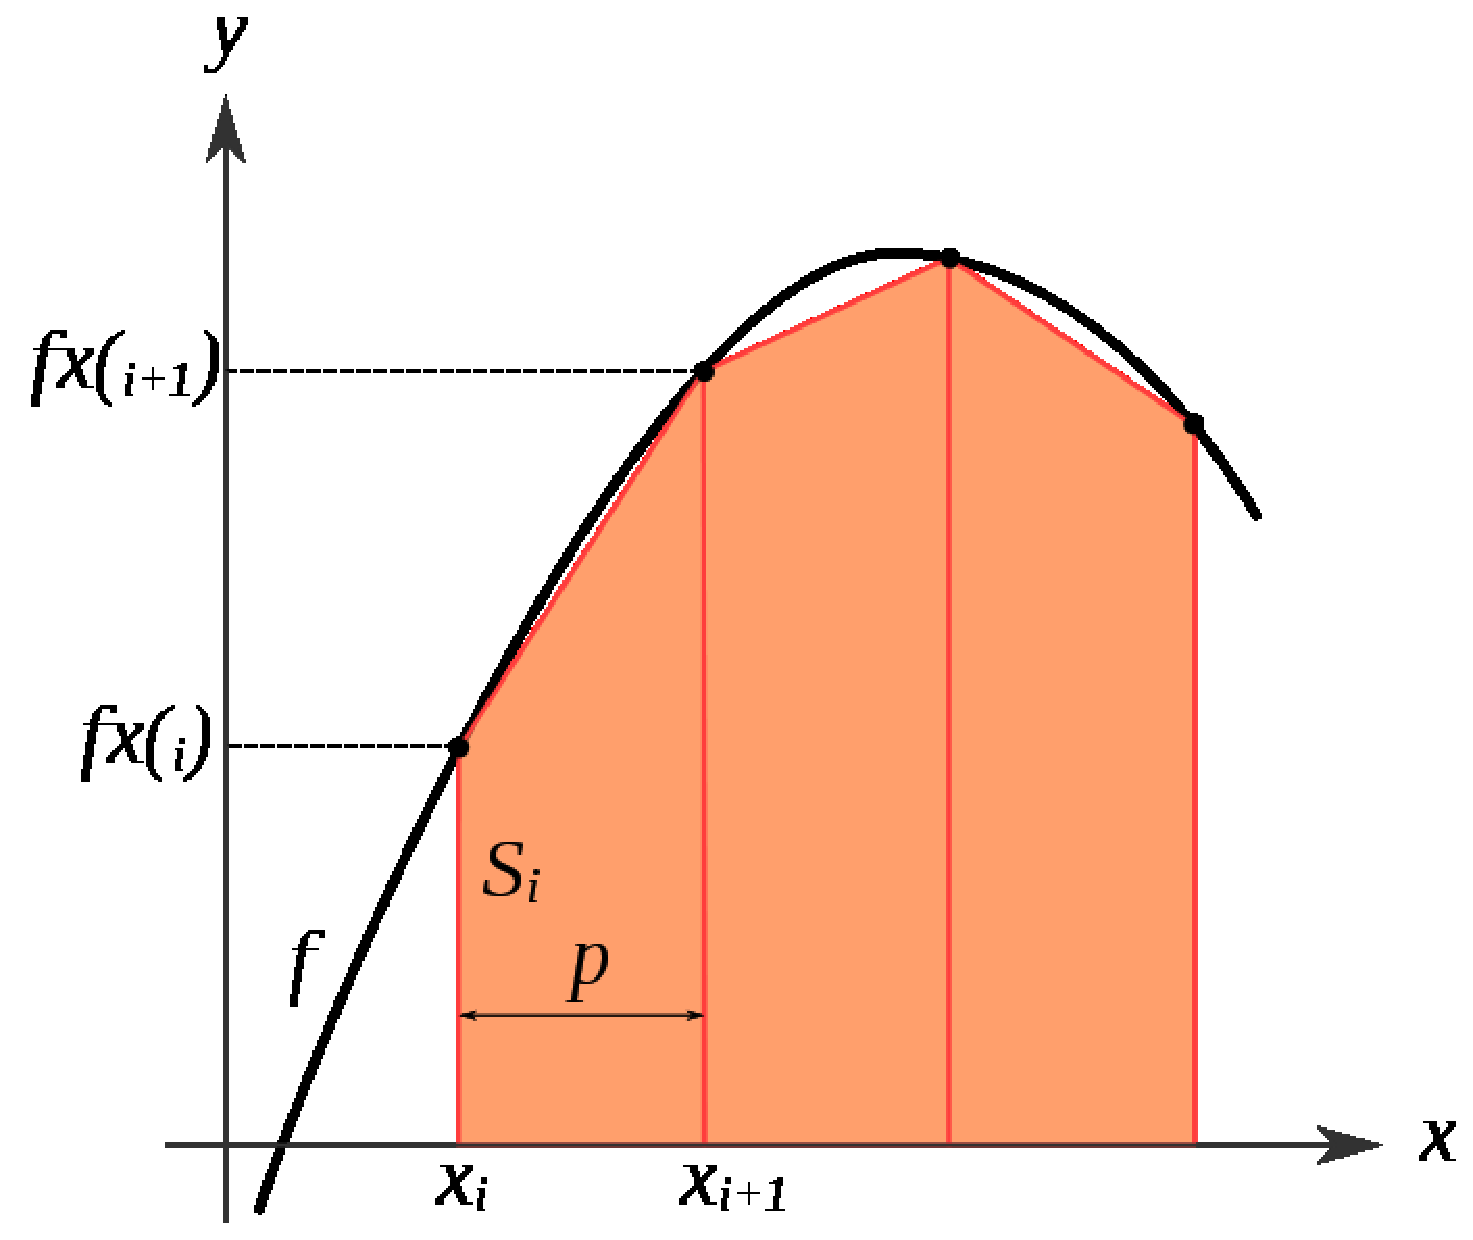
\includegraphics[width=\columnwidth]{./figs/trapezoid_wiki.eps}
\caption{Trapezoidal Rule.}
\label{fig:trapezoid_wiki}
\end{figure}
\solution  The integral can be computed as \cite{trapezoid}
%
\begin{multline}
\int_{a}^{b}f(x)\,dx \approx h \lsbrak{\tfrac{1}{2}f(a)+f(x_1)+f(x_2)}
\\
+\dots + \rsbrak{f(x_{n-1})+\tfrac{1}{2}f(b)}
\end{multline}
%
where $h = \frac{b-a}{n}$.
\begin{problem}
Solve 
\begin{equation}
\label{eq:integ}
\int_{0}^{1}e^{-x^2}\,dx
\end{equation}
using the trapezoidal rule with $n =10$.
\end{problem}
\solution The following script computes the integral in \eqref{eq:integ} resulting in
\begin{equation}
J = 0.701724989509
\end{equation}
\lstinputlisting{./codes/trapezoid.py}
\section{Simpson's Rule}
\subsection{Simpson's 1/3 Rule}
%\numberwithin{equation}{section}
%\begin{definition}
The Simpson's 1/3 rule for \eqref{eq:integ} can be expressed as \cite{kreyszig}
%\setcounter{equation}{3.0}
%
\begin{multline}
\label{eq:simpson:1by3}
\int_{a}^{b}f(x)\,dx \approx \frac{h}{3} \lsbrak{f_0+4f_1+2f_2 + 4f_3 +}
\\
\dots + \rsbrak{2f_{2m-2}+4f_{2m-1}+f_{2m})}
\end{multline}
%
where 
%
\begin{align}
h &= \frac{b-a}{2m}, f_j = f\brak{x_j},
\\
x_j &= x_{j-1} + h, x_0 = a, x_{2m} = b
\end{align}
%
%\end{definition}

\begin{problem}
Adapt \eqref{eq:simpson:1by3} into a difference equation
\end{problem}
\solution The desired equation is
%
\begin{align}
\label{eq:simpson_1_3_diff}
s_0 &= f_0 + f_{2m}
\\
s_1 &= f_1 + f_3 + \dots + f_{2m-1}
\\
s_2 &= f_2 + f_4 + \dots + f_{2m-2}
\\
h &= \frac{b-a}{2m}	
\\
J &= \frac{h}{3} \brak{s_0 + 4s_1 + 2s_2}
\end{align}
%
\begin{problem}
Solve \eqref{eq:integ}
using the Simpson's $\frac{1}{3}$rd rule with $n =10$.
\end{problem}
\solution The following script computes the integral in \eqref{eq:integ} using \eqref{eq:simpson:1by3} resulting in
\begin{equation}
J = 0.746824948254
\end{equation}
\lstinputlisting{./codes/simpson1by3.py}
\subsection{Simpson's 3/8 Rule}
The Simpson's 3/8 rule can be expressed as \cite{simpson3by8}
\begin{multline}
\label{eq:simpson:3by8}
\int _{a}^{b}f(x)\,dx\approx {\tfrac {3h}{8}}\lsbrak{f(x_{0})+3f(x_{1})+3f(x_{2})
+2f(x_{3})}
\\
+3f(x_{4})
+\rsbrak{3f(x_{5})+2f(x_{6})+...+f(x_{n})}.
\end{multline}
%

\begin{problem}
Adapt \eqref{eq:simpson:3by8} into a difference equation
\end{problem}

\solution The desired equation is
%
\begin{align}
\label{eq:simpson_3_8_diff}
s_0 &= f_0 + f_{3m}
\\
s_1 &= f_1 + f_4 + \dots + f_{3m-2}
\\
s_2 &= f_2 + f_5 + \dots + f_{3m-1}
\\
s_3 &= f_3 + f_6 + \dots + f_{3m-3}
\\
h &= \frac{b-a}{3m}	
\\
J &= \frac{3h}{8} \brak{s_0 + 3s_1 + 3s_2 + 2s_3}
\end{align}
%
\begin{problem}
Solve \eqref{eq:integ}
using \eqref{eq:simpson:3by8} with $n =30$.
\end{problem}
\solution The following script computes the integral in \eqref{eq:integ} using \eqref{eq:simpson:3by8} resulting in
\begin{equation}
J = 0.746824155509
\end{equation}
\lstinputlisting{./codes/simpson3by8.py}
\section{Generalized Quadrature}
%
The Gauss quadrature formula is given by \cite{kreyszig}
\begin{equation}
\label{eq:gauss_quadrature}
\int_{-1}^{1}f(t)\,dt \approx \sum_{j=1}^{n}w_jf\brak{t_j}
\end{equation}
where $w_j$ and $t_j$ are obtained from the Legendre polynomial of order $n$.
%
\begin{problem}
Find an expression for \eqref{eq:integ} from \eqref{eq:gauss_quadrature}.
\end{problem}
%
\solution From \eqref{eq:gauss_quadrature}, substituting 
\begin{equation}
x = \frac{1}{2}\sbrak{a\brak{1-t}+ b\brak{t+1}},
\end{equation}
%
\begin{align}
\label{eq:gen_quad}
\int_{a}^{b}f(x)\,dx  = \frac{b-a}{2}\int_{-1}^{1}f\cbrak{(t + 1)\frac{(b - a)}{2} + a}\,dt  
\end{align}
%
%
\begin{problem}
Solve \eqref{eq:integ}
using \eqref{eq:gen_quad} with $n =3$ in \eqref{eq:gauss_quadrature}.
\end{problem}
\solution The following script computes the integral in \eqref{eq:integ} using \eqref{eq:gauss_quadrature} resulting in
\begin{equation}
J = 0.746814584191
\end{equation}
\lstinputlisting{./codes/gauss_quadrature.py}

%\begin{figure}[!h]
%\centering
%\includegraphics[width=\columnwidth]{./figs/taylor.eps}
%\caption{Taylor series method.}
%\label{fig:taylor}
%\end{figure}
%
%
\bibliography{IEEEabrv,gvv_integ}
\end{document}


